“So, where’s your internship this summer?”

Looking up at Lyra, Ruth’s eyes widened. That question was something she was putting off thinking about. She looked down, returned to pulling the remaining grass from the dirt. “I applied to a bunch of places…”

Luckily, Austin cut her off. “I’m at an insurance consultancy. It should be good, but I forgot to ask for a holiday in the middle. I start as soon as-''

“Ha!” Lyra laughed, “What a noob error. As soon as they offer, you just say, like, ‘I want 4 weeks paid leave on expenses’. Milk them for everything you can get.” She sat up straight, eager to begin a lecture on ‘putting-your-foot-down’, one that both Ruth and Austin had heard before. “I’m staying at Uni in the Shock Physics group! They don’t care when I’m in as long as I answer an email once a week.”

Austin’s familiar sigh was one of defeat. “It’s a bit too late to adjust now. They have client meetings every week from June till September…”

Ruth eyed the yellow grass between her fingers. She hadn’t told anyone yet. It was hard to know how people would react – would they offer condolences? Compliments? They might even be jealous. 

Whilst Lyra resumed preaching, Ruth looked across the park, bleached yellow by the sun. The city beyond was lit up in a muddy haze. June was almost over, but the texture of the grass in her hand was more like a dry autumn leaf. It filled Ruth with nostalgia for starting term again – but that meant facing up to what was to come. She breathed out slowly, looked back down and said it. 

“I accepted a positon at Sainsburys.”

Austin stared in disbelief. Lyra squealed, threw her ice cream aside and rushed to Ruth’s side. “Really? You kept this so quiet! When do you start? What part are you working in? Is it Strategy? Management? Oh, is the pay as good as they say it is?”

It was Austin’s question that made Ruth look up from the pile of twisted grass in her lap. “Isn’t that dangerous?”

Ruth shrugged after a moment of silence. “I suppose. But, you take what you can get, right? Any experience is good experience these days.”

“But,” Lyra said, “that’s not just any experience! It’s so exciting! You must tell us what happens!”

Austin’s tone became much more critical. “How are you even qualified? And I thought they stopped hiring science students, anyway?”

“Well, you can do anything with a Physics degree these days, right?” said Ruth, slightly enjoying his reaction. Both Austin and Lyra were clearly jealous. 

“Yeah!” Lyra said, “And that’s rich coming from you, Austin – why is a Bioengineer doing risk assessments?” 

Austin rolled his eyes. “It’s an insurance consultancy I said, it’s not just risk assessments. But Sainsburys – I mean, that’s going to be such physically demanding work. Not to mention life threateningly dangerous! What division did you say it was?”

Ruth shrugged, “I didn’t. The only spot they had left was as a Deliverer.”

“No way,” Lyra squealed, “that’s the best pay grade!”

Austin was now aghast. “But that’s the frontlines! What were you thinking?” 

“I was thinking it would boost my CV and pay my rent for a year,” Ruth growled, “and don’t judge me – I saw your name on the shortlist as well.”

Austin blushed, “That’s because I was only going for the logistics summer rotation – for that, you just need to wear a bullet proof jacket on your way in. But deliveries?” He shook his head. “If it’s anywhere near any other supermarket territories, you’ll be in constant danger.”

Lyra jumped in to defend Ruth. “She can handle herself! It’s like you don’t even know her.”

“They said they only let me in because I had been playing rugby since year 10. And still I have to take a test on the Supermarket Engagement Levy-Law before I can start.” Ruth’s voice slowed as she spoke. 

Austin was finally lost for words. As they all heard ‘Supermarket Engagement Levy-Law’, the situation began to feel much more real. The stale air gave way to a breeze which plucked grass from Ruth’s lap, scattering it into the air.

Lyra watched them go, and then spoke in a stern tone, “if you think about it, that law has done so much for the world today. I mean, who knew that arming supermarkets would lead to ceasefires of all wars, worldwide, within \emph{three} years? It’s just mind boggling.”

Ruth had been reading up on this. “Essentially, all wars prior were in some way driven by the convenience industry. Sometimes not directly, but governments and energy companies would have huge stakes in the big supermarkets. They would push the sides against each other in a hope to damage the other’s stock value.”

“So,” Lyra said, “as soon as you just let them fight in the open…”

“…The wars quickly stopped,” Ruth said, as if reading from a history book. “It’s amazing that the corruption was so deep. Now, it’s in the open, and can be regulated.”

Austin shook his head. “But, at what cost? Now the war is here, in our very streets. And you’re going to be part of it.”

“Statistically, there isn’t much risk to civilians. And when there is, the government has a strict procedure to follow,” Ruth said, in the most reassuring tone she could muster. “It’s like taking the all the intense wars ruining so many lives, and sprinkling them over the whole world in a super thin layer.”

“And taxing it,” Lyra chimed in, the only one of them smiling. “It’s beautiful, don’t you think?”

Austin opened his mouth to speak, but swallowed his questions quickly when he saw Lyra’s scowl.

“It’s okay, really,” Ruth put her hand on Austin’s knee to show she was being sincere. “I sign a NDA for getting to see some of the command centre, but not my soul away with the full contract. I’ll be absolutely fine, I can handle myself.”

“Where are you based, then?” Lrya was keen to get back to her long list of questions.

“Their territory is mostly in the south east, but they put me in Reading.”

Austin spoke again, his voice barely there. “But that’s Waitrose territory. Right? My dad lived there for a few years. They control all the ring roads, petrol stations and have a distribution centre right in the middle.”

Ruth’s stomach sank as he spoke. “Oh – well, that doesn’t seem right for a first timer. Maybe I can ask for a transfer?”

Lyra sank a little too. “Yeah. Just, uh, put your foot down. Go somewhere quiet. Like Slough. I heard it’s quiet there. Maybe Swindon.”

---

Ruth gazed up at the monolithic sign, slowly reading it again and again. “Sainsburys Reading Command Centre”. Dark figures shifted on the wall above. The solid metal gates were gradually opening, revealing a busy compound, lined by lorries and delivery vans. In the centre was a huge grey building, a concrete block fortified even further with its own guard towers.  A helicopter was landing on its roof. 

A bump from behind snapped Ruth out of her trance - other workers were barging their way through. She stood aside as a crowd in dark blue boiler suits trudged through the gap in the gate. Not a single one looked up. Ruth reached into her pocket for her ID badge and pinned it to the uniform that covered her Kevlar vest. She joined the end of the line, falling into step with their dirge-like pace. 

Once through the gates, the line continued to the security office, which was little more than a brick shack with an open front. She hoped they had got the memo about her arrival. An urgent terror gripped her as she reached the front of the queue. 

“Your papers, please,” said the security guard in the shack without looking up. She sat on a swivel chair and thumbed through a long list of staff. The shack was almost completely bare, except for the back wall, on which an automatic rifle was hooked. Ruth held out her ID with a trembling hand. The guard snatched it and squinted at it. “New kid, huh,” she muttered, slowly ticking a box on the sheet. She tossed the ID back over the table, then looked up to meet Ruth’s petrified gaze. “You know what you are doing? Got your tags?”

Ruth nodded, lifting her hand into her shirt to pull out the silver tags which hung on her neck. They listed her name, blood type and organ donor number. Her unique employee number was at the top, the last letter of which stated her preferred funeral procedure, chosen from burial (B) or incineration (I). Ruth had just clicked “I’m feeling lucky” on the form, so it listed both. 

The officer grunted and turned back to the personnel sheet. “Says here you’re to report to the delivery bay and get going. First dispatch goes out at six thirty.” 

Ruth nodded, picked up her card, and shuffled away from the shack. Her watch said it was already six twenty-five. She broke into a run, kicking gravel high behind her, as she had vowed not to be late on her first day.

\begin{figure}[h!]
\centering
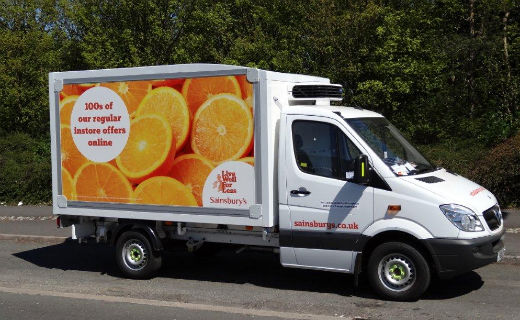
\includegraphics[width=0.7\textwidth]{./pictures/van_small}
\end{figure}

The loading bay was under the south corner of the central building. A row of delivery vans was being tended to by swarming workers. Ruth stopped running when she got to the front van and collapsed on its bonnet to catch her breath. The front was fitted with a reinforced bumper, the sides were thickly plated, and the windscreen was blacked out. On its side was a picture of a basket of blueberries and the words “One-hour delivery straight to your door!”. She looked around for someone in charge, but all activity appeared to be autonomous. 

A loud growl startled her as the van’s engine came to life. She looked up at the tinted window and barely resolved a dimly lit figure in the driver’s seat. It made some sort of hand signal at her. Ruth carefully stepped round to the passenger door and it opened before her.

A woman in the standard issue beige delivery uniform stared at Ruth from the driver’s seat.  She reminded Ruth of some of the most fearsome fullbacks she had been tackled by in her time. She had one hand on the wheel and the other on the gearstick - in her grip, it looked more like a ballpoint pen. 

She spoke slowly in a low voice. “I’m Morgan. You’re Ruth. Get in.” 

Ruth stepped almost a meter up into the vehicle and sank into the seat. The reinforcements and adjustments made the interior very small, making her feel like she was being pinned against the window. Morgan flipped a switch on the busy dashboard and the door slammed shut behind Ruth, followed by loud whirr could only have been the lock mechanism. The air smelt of engine grease and Pot Noodle. 

Ruth swallowed her fear, strapped in, and spoke in the most determined tone she could muster. “So - what’s the plan?”

“I drive, you watch. We deliver,” Morgan said without delay. She went into first gear and hit the gas. Within moments, the van was through the gates, its precious cargo rattling in the back. 

---

Their headlights lit the streets in a sickly orange tone. The suburbs they drove through were barren and empty. The two hadn’t shared words for minutes. 

Ruth took the time to study the instruments in front of her. A green dot blinked on a screen near the centre of a map, showing their location, and an orange line traced their route ahead. Morgan didn’t seem to be checking it or even following it, as she had her own clipboard with addresses hanging to her right. Ruth seemed to therefore just be in charge of a communicator, currently buzzing faintly with static. 

The silence quickly became unbearable. “Anything I should know?” Ruth asked.

“Hmm,” Morgan hummed, either irritated or bemused. “You tell me - what should you be doing right now?”

Ruth had memorised the handbook of procedures. “I navigate. Watch for hostile vans. Unload. That sort of thing.” Now that she was locked in the car and on the move, some of the tension had been defused. Morgan seemed experienced, so she felt like she was in safe hands. “Will there be a test?”

Morgan didn’t seem to laugh. “It’s too late for tests now. Just do what I say.”

Ruth nodded, and tried to forget the other jokes she had prepared to break the ice, but they all crammed into her mind at once. Sadly, the melody for ‘the wheels on the van go round and round’ was really catchy. “Right. Whatever you say. You been doing this for long?”

Morgan didn’t respond until they turned onto a busy dual carriageway. Their van towered over the other cars, which almost seemed to part to clear the way, as if delivery vans were emergency vehicles. “Yes. Three years.”

Ruth’s eyes widened. Three years on this salary was long enough to save for a comfortable life, not to mention pension and retirement. 

“Damn, this is new,” Morgan muttered as orange roadworks signs began to appear on both sides of the road. “Okay, looks like your first job is to find us a new route. Use the map, and avoid everything south of Oxford Road.”

Ruth pulled the screen up and strained her eyes at the mess of moving dots. “Which one is...”

“We are green. Target is the red circle.”

“Uh, right,” Ruth stammered, looking now at the intricate mess of one way arrows on at least half of the roads. She traced a possible route with her finger and the system began to adjust its auto-route for her. “Left here.”

The van lurched left, now going down a side road, just before a wall of idling traffic cut off their original route. Ruth only just managed to keep on track of issuing Morgan with directions, let alone scanning the roads for other vans. “On this round about, third - no, second exit. Second.” Other questions invaded her mind. “What sort of aggression policy is in place here?”

Morgan’s voice gave away how irritated she was getting at the sketchy directions. “Protocol 25 B. You should know what that means.”

“Yes, absolutely,” Ruth replied. 25 B meant that when rival supermarkets met whilst out on delivery, they were allowed to ‘disrupt one another’s activities’, but they couldn’t seek each other out or murder rival Deliverers. Additionally, the only violence allowed was Deliverer against Deliverer – other roles weren’t supposed to interfere or become at risk. The Sainsburys rulebook had explicitly stated the following: “It is still entirely appropriate to shoot hostile Deliverers in these zones, but please ensure shots land on armored areas of the target’s body such that they are not significantly maimed to cause accidental death”. It didn’t really matter to Ruth, because interns were not given guns. Ruth wondered what Waitrose’s handbook said.

The van slowly halted at a red light. Traffic zoomed in front of them from right to left whilst they waited for their turn. Ruth attempted to look for hostile vans, but the murky light, the vehicles became a blurred mass. Paranoia began to grip her too - any remotely large vehicle rang alarm bells as it thundered past, be they bland and white, or carrying other brand names, like DHL or the Post Office. 

Morgan tapped impatiently on the wheel as the lights changed again to let pedestrians cross, leaving the junction open. “We better not be late after this. Is it right or straight ahead?”

“Oh,” Ruth said, looking back down at the map, “It doesn’t really matter, because-”

“Damn it,” Morgan snapped, “I didn’t ask for a smart answer!”

“Then go straight!” Ruth shouted - though she didn’t intend to say it so loud. Morgan turned her scowl upon her and opened her mouth to return the favor, but the red light turned orange in that moment. She returned her eyes to the road and hit the accelerator hard. Ruth turned away in shame to look at the traffic waiting to go at the other lights. She saw a silver blur moving quickly towards them.  

They were barely halfway across when it hit them. 

Before she could duck down, the window glass shattered over her face. Morgan swerved the wheel to fight against the massive impact, and then bolted from her seat out on the crossing. The van lurched to a halt.

They’d been rammed by another van. Ruth kept her head down, listening to the opposing drivers open their doors. Through ringing ears, she heard one yell, “I’ll take the navigator! You get the driver!” She froze up and stared wide eyed at her knees, waiting for the inevitable. It was her fault entirely – that van must have been in view for at least a few precious seconds. 

The door was yanked open and she turned to see man wearing an orange hi-vis kelvar jacket emblazoned with the word “Ocado”. In the hand not pulling back the door, he was raising a stun baton that sparked with energy. But before it could strike her, a loud bang rang in Ruth’s left ear – a gunshot. She blinked and the Ocado Deliverer was down, clutching his chest and groaning. 

Morgan stood with a pistol raised at the other van. “Stay down!” she screamed at Ruth, scanning for the second Deliverer – but they were nowhere to be seen. She crept forwards to check all sides of the Ocado van. By now, pedestrians and drivers were watching in bemusement and horror, some with their phones out. 

Ruth watched Morgan tiptoe around the back of the van. Cars were honking far away as the morning commute was fatally disrupted for many. As soon as Morgan was out of sight, Ruth felt truly alone, as if the busy traffic and onlookers had faded away.  

\begin{figure}[h!]
\centering
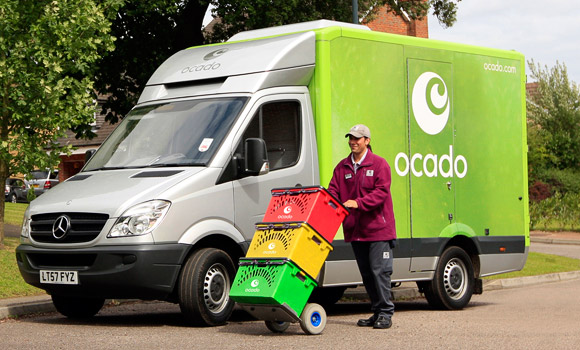
\includegraphics[width=0.7\textwidth]{./pictures/ocado}
\end{figure}

The missing Ocado Deliverer emerged from behind the front of his van. He made run for the body sprawled in front of Ruth’s open door. He didn’t even look up as Ruth slowly rose from her seat. He was much more concerned about the state of his co-Deliverer. In a panicked rush, he fell to his knees by the other’s head. “Christ, Dave! Are you okay?” he whispered.

The floored Deliverer coughed and nodded slowly. “It’s just my rib, my vest caught the bullet”, he said weakly, then raised a finger upwards – “Go get the gun!”

The other nodded, then rose. Ruth saw her chance and her instincts flared. 

She threw herself from the seat and collided with the now standing deliver’s legs. She hit his shins with her shoulder, and in an instant the fight was over. Most rugby players knew instinctively how to fall – but he just toppled like a tower of cards. The back of his head hit the wing mirror of the Ocado van on his way down. Ruth winced at the sound, hoping it was the glass she heard crack, not his skull. 

Morgan came running out from behind the Ocado van to see Ruth standing over the two bodies. “Good job,” she said, “now get back in the truck.” 

Ruth didn’t need to be told twice. In a flash they were both back in the idling van. Clearly, these vehicles were built for such impacts, as the only signs of damage were paint scratches, a slightly buckled side door and the passenger seat’s smashed window. She got into the seat, shut the door and said “I’m sorry – I wasn’t looking out for Ocado vans. I forgot that they’re partners with Waitrose…”

Morgan jumped into the driver’s seat just as fast and revved the engine. If she heard Ruth’s apology, she didn’t seem to care. “Before we go, hit the button with an ‘S’ on it.”

Ruth nodded grimly, knowing exactly what it did. She pressed it with a shaking hand, making the speaker on the top of the van crackle into life. She glanced at the two Ocado Deliverers groaning on the floor as the classic Sainsburys jingle began to play. “Live well for less” echoed down all the nearby streets, signaling that they had won this encounter. The traffic parted and the van rolled onwards. 

---

The rest of the drive was completed in silence, allowing both Ruth and Morgan to catch their breath. Ruth just had to point to where they needed to pull over to make the delivery – a quiet side road, lined by terraced houses on both sides. Morgan was the first to break the silence once she had finished pulling in. “You know kid, you did good. Real good. I couldn’t ask for more. Sorry I snapped at you at first.”

“Oh, please, it’s okay, I don’t mind,” Ruth said in a flurry, “I understand. Well, of course, I don’t understand, I could never really… I can’t imagine doing this for three years like you!” 

“I don’t do that every day, don’t worry” Morgan laughed, “Maybe once a month. There’s plenty of boring to go with the thrill.”

Ruth smiled. “Speaking of which should we, uh, deliver?” 

Morgan left the van and pulled open the door to the storage compartment. It creaked on its hinge, a reminder that the previous encounter hadn’t just been a bad dream. “Delivery is for…” she mumbled as she scanned her clipboard, “number 24. This crate.” 

Ruth pulled the heavy box out. The order included fruit, dried pasta, cornflakes (Sainsbury’s own brand), and some toiletries. She hauled it to the doorway where Morgan was now standing, hammering the buzzer. Ruth suddenly appreciated how much taller and broader Morgan was than her.

The door sprang open and the face of an old lady smiled back. “Oh, it’s my order! Hello Miss Morgan! Thank you dears, if you could please bring it to my kitchen, follow me, you know, these £1 delivery slots are just a bargain…”

Morgan grunted, “You go in Ruth. I’ll wait,” standing back to let her through. “Heh, three years and I’m no good with customers. Or old women…”

The smell of earl grey filled her lungs as Ruth stepped into the hallway, following the shrill sound of the customer. Knitted doilies in mostly beige colours were draped over the furniture. The carpet was incredibly soft underfoot, as if it was itself carpeted with a thick layer of cat fur. The kitchen was tiny, and the table only just had space for the huge blue crate. However, everything was neat, and once the woman had stopped talking, the serene quiet of being away from the streets was incredibly comforting. 

“I’ll give you a hand unpacking,” the old lady said, leaning over the box to grab a bunch of bananas. “Just follow the labels. Fruits on the shelf over there. I’ve not had you come and deliver before, dear, are you new?”

“Uhm,” Ruth stammered, “Yes, I’m an intern. Only for 6 weeks.” She mulled that thought around her head. 6 weeks to go, and even in the first hour they’d already shot someone. 

“Oh, you’ll do very well, I’m sure, and get a nice bit of pocket money too. Jill at church has a daughter who’s interning at Marks and Sparks…”

The unpacking took several long minutes, because each item Ruth picked up needed to be cross checked against all the little notes the lady had in her kitchen. Questions stumped Ruth that she hadn’t even thought she’d have to consider in a job like this. Do the Jaffa cakes go in the biscuit or the cake tin? 

As the pile got smaller, the old woman changed tone, “Oh, dearest, I’m sorry but I think I’m missing my Werther's Originals.”

Ruth turned and was lost for words. “Oh. Right,” she said, “I’ll just, uh, check with Morgan.” She put the Jaffa cake box into the woman’s empty hands and dashed out of the room. This sort of situation wasn’t in the manual.

Morgan was standing by the van with a hand on her gun, looking left and right along the street. “Problem?” she asked as Ruth stepped close enough to whisper in her ear. 

“Missing something,” she hissed, “Werther's Originals.” 

Morgan gazed back in shock, then turned and slammed her fist on the van. “Damn it! But I checked the cargo myself! You sure they’re missing?”

“Uhm, well, old ladies tend to notice when it’s Werther's Originals,” Ruth said with a snigger, but instantly regretted it when Morgan turned her angry gaze back.

“This isn’t funny! You know what happens now?” Morgan said in an angry whisper, “I get sent before the line manager! They come down on these mistakes hard. Last time one of the haulers got fired!”

Ruth cowered back, retreating to her mind in the hope of finding a solution. The old lady was standing on the doorstep again, smiling, seemingly unaware of the gravity of the situation. Ruth turned back with a hopeful grin, a plan formed. “Look, we can fix this. We just find a shop nearby that sells them and chuck them in the crate. Nobody at central needs to know.”

Morgan shook her head. “You don’t know the area. There’s no Sainsburys Local for miles. We have 10 more deliveries to do, we don’t have time…”

“But what about another supermarket?” Ruth said, pulling open the passenger door to look at the screen. She recalled there had been a skull-and-crossbones marker very close to this street. “Look, there’s a Little Waitrose just on the next street!”

The old lady piped up. “Yes, there is, but it’s not very good, they have those machines which beep at you when you try to buy loose vegetables…” 

\begin{figure}[h!]
\centering
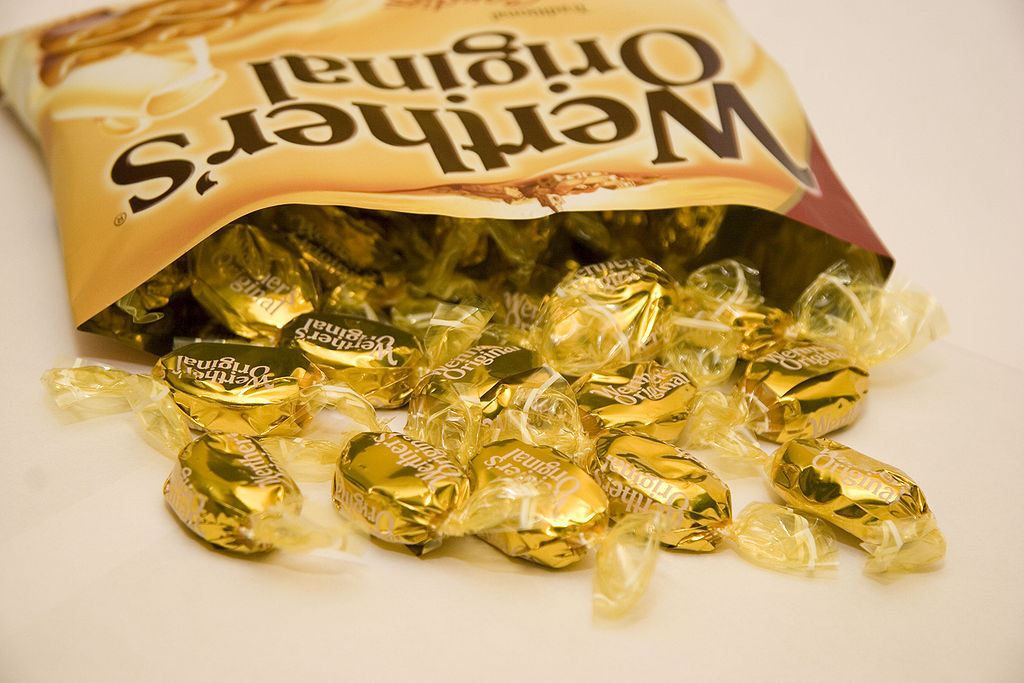
\includegraphics[width=0.7\textwidth]{./pictures/originals}
\end{figure}

Morgan leaned closer and gripped Ruth’s sleeve. “No, you don’t get it. I’ve been at this gig far too long. They all know me, they have my picture on file. I can’t go in.”

Ruth looked back in surprise. “Well, that’s fine. I’ll go.”

“No!” Morgan shouted. The old woman stopped talking behind them and backed into her hallway again. “Ruth, I can’t let you. It’s not worth the risk. They might have got your details, they could get you as soon as you walk in.”

“What do you mean? I’ll just take off my vest. How can they know who I am? It’s my first day!” 

“I mean, it’s not safe!” Morgan hissed. Ruth could tell there was more to this – Morgan was very easy to read. What wasn’t she telling her? “It’s never safe. Please, don’t do it. I’ll just take the punishment.”

Ruth shook her head. No way would she let Morgan take the heat for this. “I’m sorry. I can’t let that happen. I’ll be back in 5. Just stay here and watch the van.” Ruth tore off her jacket, thrust it towards Morgan, then dashed off down the street. 

She ignored Mogan’s frantic cries as they faded behind her. “Wait! Don’t…”

--- 

The ‘little’ Waitrose was particularly little, nestled under a four-story block of flats on the street corner. It was flanked by two 
security guards, wearing sunglasses (despite it being 7am and overcast). Ruth was puzzled when she noticed a line of customers trailing out of the front of the shop onto the street, but upon closer inspection, they were all waiting for a spluttering self-service coffee machine to cough back to life. She slowed to a walk and tried to blend in. 

She passed the guards with her head down. She didn’t raise it again until she was on the confectionary isle, which she found through pure instinct. Maltesers… Double Deckers… Yoghurt-covered raisins… Werther's Originals! She took two bags for good measure and peeked up towards the checkouts. 

There were two self-check-out machines, and two staff operated tills. She made for the self-check outs, but she accidentally caught the gaze of a server at the staff tills. “Hello ma’am, can I ring those up for you?” 

Ruth looked away, pretending she didn’t hear, and went straight to scanning on one of the self-scanners. The machine’s screen flickered ominously with the Waitrose logo. She wasted no time scanning the sweets, then searched for her wallet with shaking hands. A loud ‘clonk’ sound came from the coffee machine – somebody must have kicked it. Ruth scanned her card and watched the screen intently, waiting for the “contacting your bank” message to clear. 

…but did it usually take this long? Ruth looked around the room again. The looked back at the staff tills, but the server there was gone. She began to consider running off with the sweets, cursing herself for bothering to pay in the first place. If she made a break for it now, her cover would be blown. Ruth could feel her heart beating in her throat. Finally, the screen finally changed message. 

“There is a problem with your purchase. Please consult a member of staff.”

Before Ruth could run, a faint ‘click’ sounded next to her ear. She turned to look down the barrel of a handgun, held by the person who had been running the tills. Her heart dropped and she froze, glaring at the same smiling face. 

The server, whose name tag read ‘Bridget’, kept her gun raised. In the other, she activated a bulky handheld receiver and spoke, “Commander, we’ve got a Deliverer who doesn’t know where she’s welcome. Please send up a truck. Cheers, love.”

Ruth thought fast. Distraction. She had moments before the guards at the entrance would be upon her. If she was going to move under a loaded gun, it needed to be right at this moment. 

Suddenly, a loud smash sounded from the other aisle, followed by cheering from the line for the coffee. Bridget winced, “Oh, blast! Not again!”

Ruth turned to run, but the server was ready. As she attempted to make her second step, Bridget’s leg smashed into her foot, which instantly sent her spinning to the floor. Ruth’s cheek hit the tiles. Bridget knelt with her knee firmly on Ruth’s shoulder and held the pistol at her temple again. “You’re really not smart are you, poppet?” Her reciever buzzed to life, a grainy voice speaking through it, though Ruth couldn’t make out a single word. “Oh, did you hear that, dear? Ocado got your partner. Not smart to park a street away.” 

The pain on her face faded away slowly as a wave of coffee trickled towards her. In the other aisle, the door guards were pulling people away from the self-service machine, which was emptying itself relentlessly onto the floor. By the time her blood on the floor mixed with the cold coffee, she had blacked out. 

--- 

“Ruth! Wake up, damn it!”

Ruth jolted awake to complete darkness and a splitting headache. Her hands were cuffed behind her back, attached to the railing of the bench she was sat on. All around her the walls shook – she was in a vehicle. To her right, a familiar voice barked, “Are you alright? Answer me damn it!”

“Morgan? I’m fine!” Ruth said. She felt a lump on her cheek ache as she spoke. “Tell me what the hell just happened!”

Morgan’s voice shifted closer to be heard over the rumbling engine. “They put us in the Ocado van. The same guys from earlier.”

“I worked out that much! How did they work out our location?” Ruth said. 

“They tracked your credit card, and linked you to Sainsburys,” Morgan sighed. “That must have set of alerts everywhere, because the Ocado thugs were hunting us and showed up straight away.”

Ruth sat back, reeling. What a first day. They were silent for a while whilst it all sank in. The pain didn’t get any better. “Wait, Morgan. How the hell did they trace my card?”

With a heavy sigh, Morgan said, “I’m an informant. For Waitrose. Not proud of it, but I do it to survive.” 

“What?” Ruth yelled, raising her voice further, “You sold me out?”

“It’s not like that. Let me explain,” Morgan began, “You stay in the game for as long as I have, you get visited by these guys. They call them ‘Bounty hunters’. They find where you live, which is supposed to be top secret, even to the supermarket you work for, then they make you cough up intelligence. It could be employee databases, strategic weaknesses, or trade secrets. If you don’t get the data, they sell your address to some other supermarket who come and take you out. That’s why a lot of people end up with broken legs.” 

“That’s…” Ruth was lost for words. 

“If you do get the data, they sell that to other supermarkets instead, and come back next month for more. And it’s legal because they’re independent – or so the supermarkets claim.”

“…utterly barbaric.”

Morgan managed a small laugh. “Yes, at the very least. But these companies can get away with anything because they’re so big. Too big to fail. Anything that increases their share prices is a price worth paying, and those of us on the frontline pay the price.”

Ruth was horrified. She let her anger out loudly, “We’re just pawns, then! They don’t give the slightest damn about any of us!” You should have shot those Ocado guys dead.”

“NO!” Morgan yelled, “I didn’t kill them because I’m a \emph{decent} human being.” Morgan’s tone changed, as if reciting a promise that she had sworn to herself. “People think Deliverers, shelf stackers, all of us, are just playing along with the cooperate game. They think we don’t deserve respect for what we do, the sacrifices we make. Mindless drones, facilitating capitalism, one falls and another takes their place. But we don’t hate each other; we don’t want to kill one another – we’re just trying not to get fired every day.” 

As she finished, the engine noise calmed and the van came to a halt. The driver doors opened and their footsteps could be heard coming to the backdoor. 

Ruth whispered to Morgan, though she knew the answer already. “So, where are we now?”

“Their HQ. For questioning. Oh Ruth, I’m so sorry…”